\begin{center} \textbf{\huge Results} \end{center}
To evaluate the performance of our classification approaches we used the cumulative accurency per interval and the cumulative accurancy over all points which are at this time not in the training set. The batch/ offline szenario performs similar the first two test phase with but seams decreasing in the last interval.

 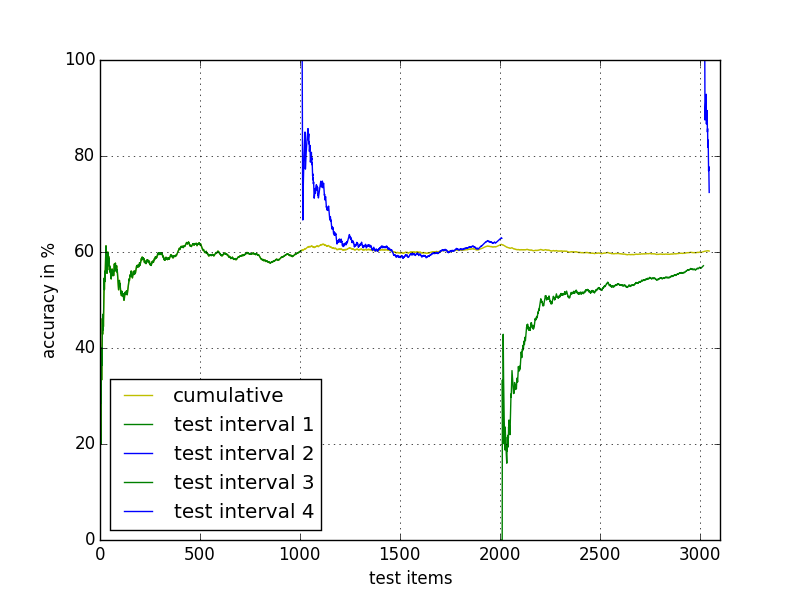
\includegraphics[width=0.2\textwidth]{./plots/batchPlot.png}\\

In the second szenario we applied the bruteforce model which rebuilt the model in the beginning of every interval.\\
   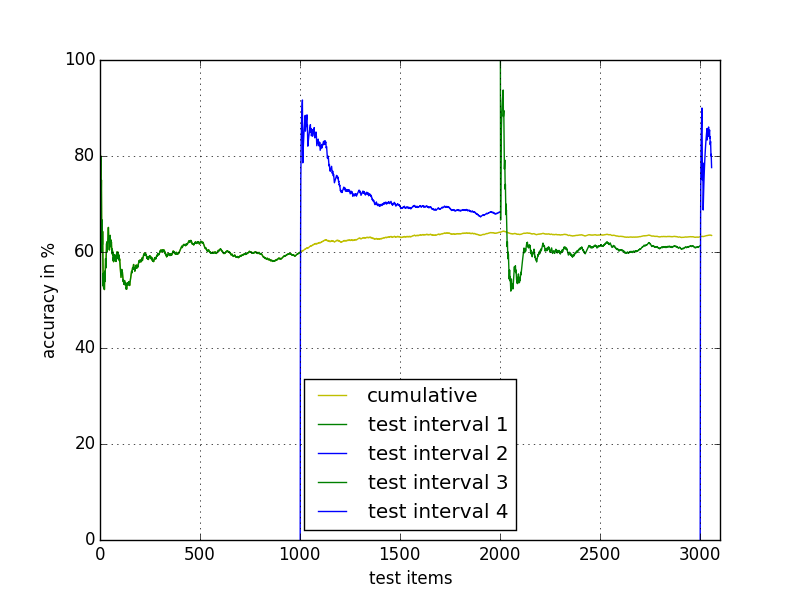
\includegraphics[width=0.2\textwidth]{./plots/bruteforce2_Plot.png}\\
In comparison with the batch version the bruteforce model gets higher accuracies in the intervals.\\

For the error-triggered model we set a threshold at 63\% of accuracy at which the model is recreated. Since we included a sanity point set the rebuilt takes place three times after the 300 sanity points and stays then constant for 1380 points after which two retraining phases follow.\\
   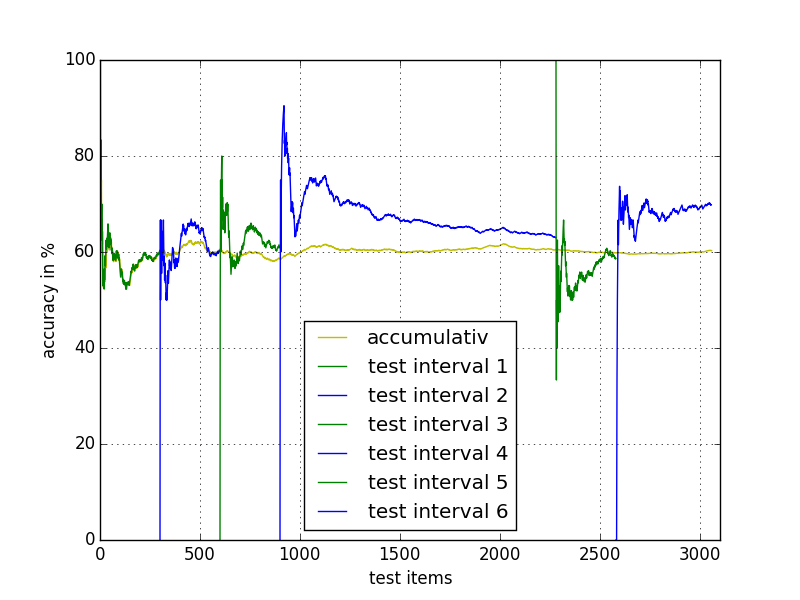
\includegraphics[width=0.2\textwidth]{./plots/errorTriggeredPlot}\\
In comparison batch and error-triggered the error-triggered has higher interval accuracy but due to the short retraining intervals avaraged they are similar. \\

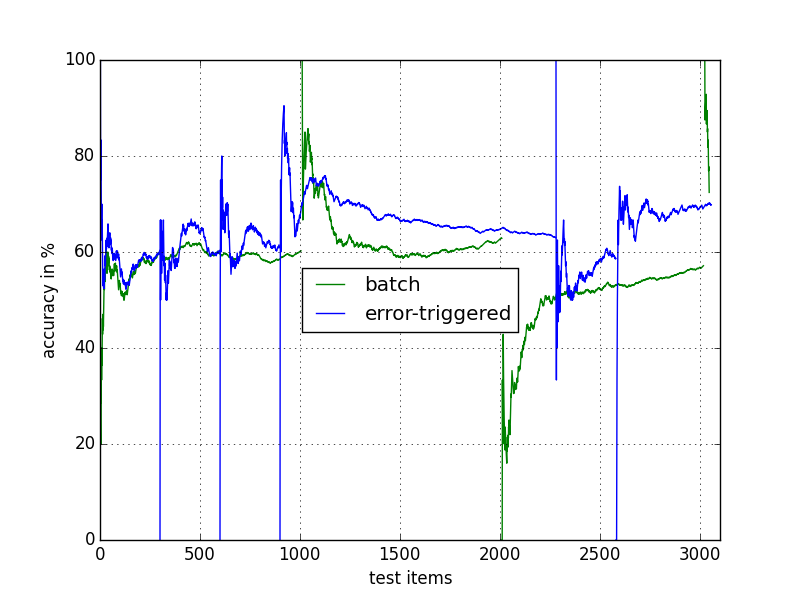
\includegraphics[width=0.2\textwidth]{./plots/errortriggered_batch}\\
Despite bruteforce and error-triggered methods have both higher interval accuracies around the phase of testpoints 1000 to 2000 which might be caused by concept drift. 
\\

The incremental one 

   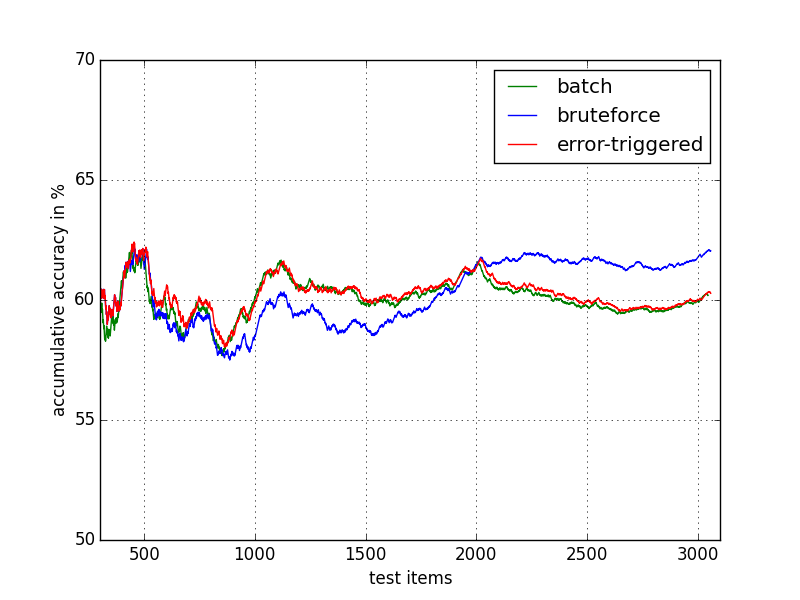
\includegraphics[width=0.2\textwidth]{./plots/allAccuracies}\\

